\section{Part A}

\subsection{Ground resonance curve}

In Fig.\,\ref{fig1} one can see the amplitude around the ground frequency of the reed, in Fig.\,\ref{fig1} the corresponding phase. Because there is a visible phase shift from 0 to $\pi$ we can say that this is definitely a resonance and not a noise peak. A Lorenzcurve
\begin{equation}
	 \frac{A_0}{\sqrt{(\omega_0^2-f^2)^2+\gamma^2f^2}}
\end{equation}
has been fitted to this data, where $f$ is the frequency, $A_0$ the amplitude of the peak, $\omega_0$ the resonance frequency of the reed and $\gamma$ the damping constant. This fit can be seen in Fig.\,\ref{fig2}. The fit is in quite good agreement with the data, giving a reduced $\chi^2$ of 1.33 which in turn gives a fit probability of $P = 10\%$. The small deviation from one is not unusual because of the high sensitivity of the system to external noise sources. The residuals, that can be seen in Fig.\,\ref{fig2} do not show a significant trend. From the fit we get $\omega_0 = 319.436\pm0.008$ and $\gamma = 5.472\pm0.014$. This then gives us a quality of
\begin{equation}
	Q = \frac{\omega_0}{\gamma} = 58.38\pm0.15
\end{equation}
using
\begin{equation}
	\delta_Q = Q\sqrt{\left(\frac{\delta_{\omega_0}}{\omega_0}\right)^2+\left(\frac{\delta_{\gamma}}{\gamma}\right)^2}
\end{equation}
and 
\begin{equation}
	\omega_R = \omega_0\sqrt{1- \frac{1}{2Q^2}} = 159.706\pm0.004
\end{equation}
using
\begin{equation}
	\delta_{\omega_R} = \sqrt{\left(\sqrt{1-\frac{1}{2Q^2}}\delta_{\omega_0}\right)^2+ \left(\frac{\omega_0}{Q^3\sqrt{4- \frac{2}{Q^2}}}\delta_{Q}\right)^2}
\end{equation}
By taking the frequency difference between the maximum and the minimum of the $A\cos(\phi)$ graph (Fig.\,\ref{fig3}) one can also calculate the quality Q
\begin{equation}
	2 \Delta f \approx \frac{\omega_R}{Q}
\end{equation}
which yields $Q = 53.24$ which is of the same order as the value that has been calculated above. Also the position of the zero of the $A\cos(\phi)$-Graph roughly conincides with the one from the amplitude peak.



\begin{figure}[h]
	\centering
	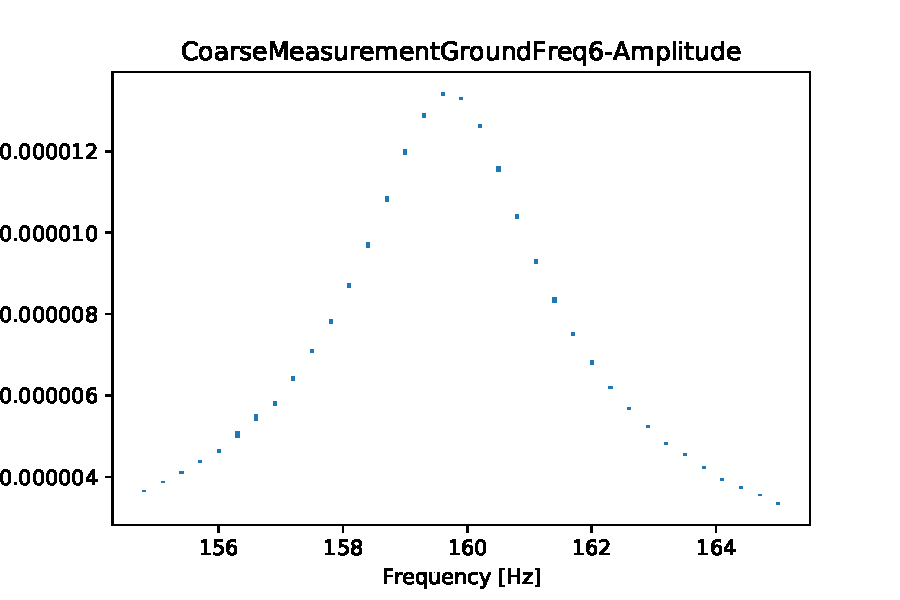
\includegraphics[width=0.45\textwidth]{figures/CoarseMeasurementGroundFreq6amp.pdf}
	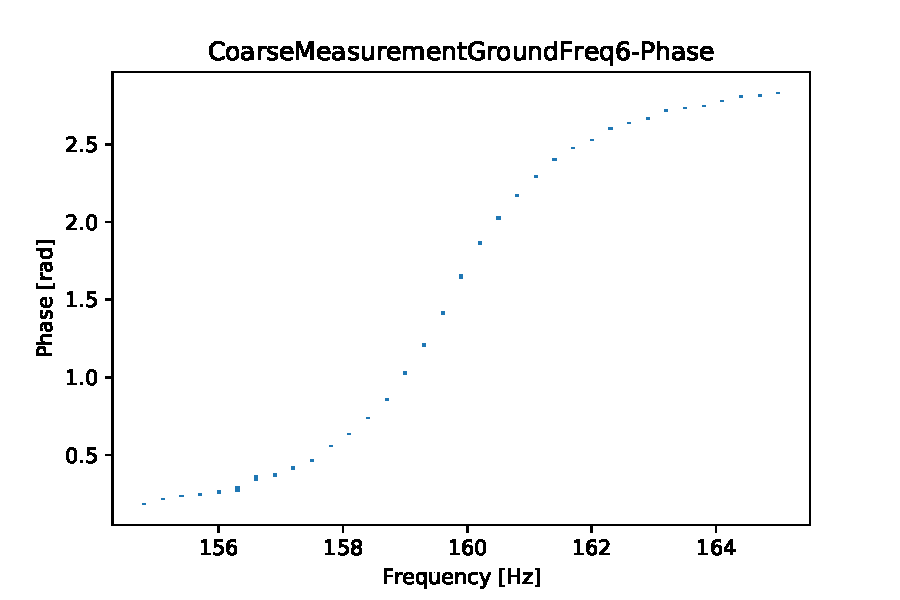
\includegraphics[width=0.45\textwidth]{figures/CoarseMeasurementGroundFreq6phase.pdf}
	\caption{\emph{Left:} Measurement of the amplitude around the ground frequency, \emph{Right:} Measurement of the phase around the ground frequency}
	\label{fig1}
\end{figure}
\begin{figure}[h]
	\centering
	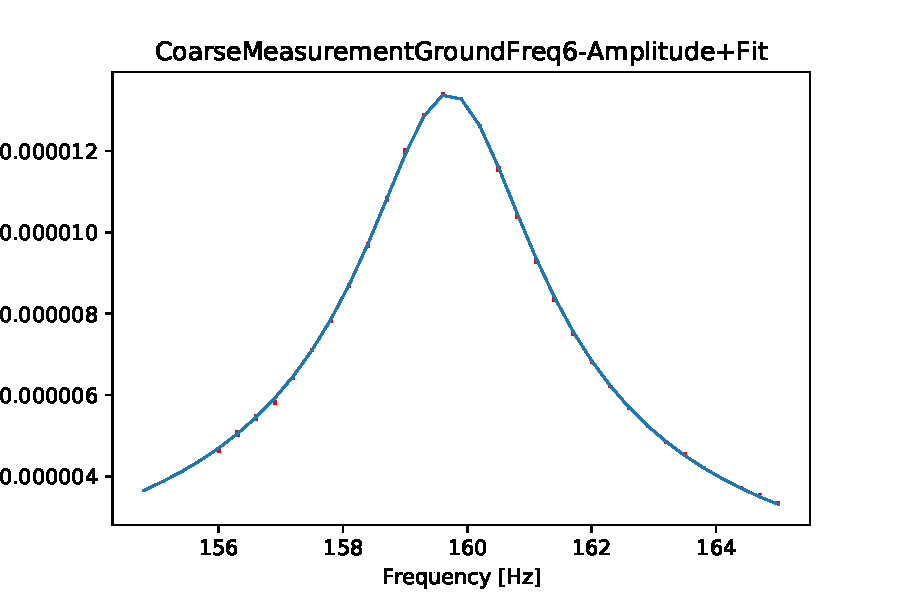
\includegraphics[width=0.45\textwidth]{figures/CoarseMeasurementGroundFreq6fit.pdf}
	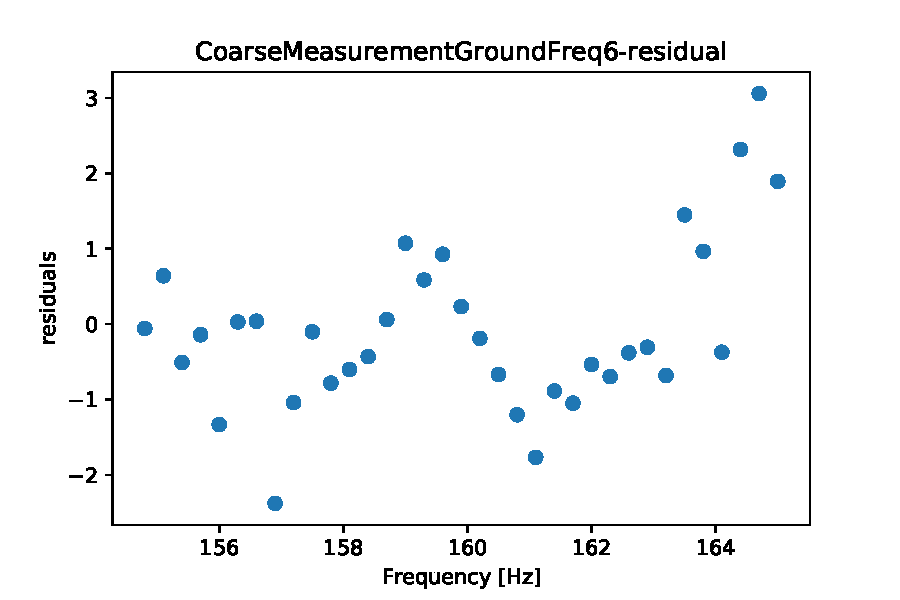
\includegraphics[width=0.45\textwidth]{figures/CoarseMeasurementGroundFreq6residuals.pdf}
	\caption{\emph{Left:} Lorenz-fit to the data, \emph{Right:} Residuals}
	\label{fig2}
\end{figure}
\begin{figure}[h]
	\centering
	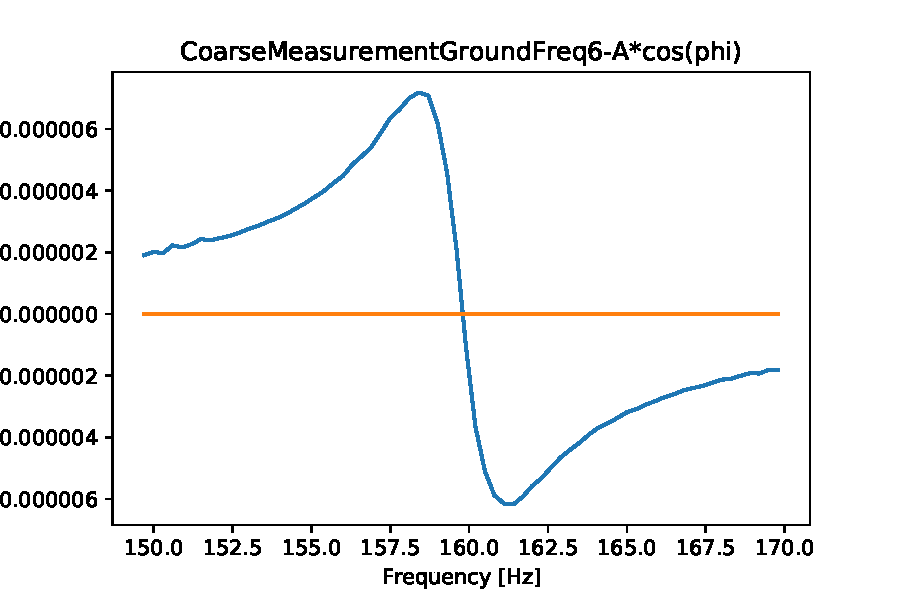
\includegraphics[width=0.45\textwidth]{figures/CoarseMeasurementGroundFreq6acos.pdf}
	\caption{$A\cos\phi$}
	\label{fig3}
\end{figure}

\subsection{first order resonance curve}
Using the same methods as described above we get the following values for the first order resonance peak.
This time the fit does not work as well as before with $\chi^2 = 2.37$ this might be because of even higher sensitivity to noise and the reduced amplitude of the second order signal. This yields a fit probability of $0\%$, which can be explained as above. Systematic error sources just play too big of a role in this case. Visually the fit works quite well though. Also the residuals do not show a significant trend (Fig.\,\ref{fig5}). From the fit we get
\begin{equation}
	\omega_0 = 1988.18\pm0.22; \,\,\,\,\,\, \gamma = 15.9\pm0.6; \,\,\,\,\,\,Q = 125\pm5; \,\,\,\,\,\,\omega_R = 1988.15\pm0.22
\end{equation}
from Fig.\,\ref{fig6} we also get $Q = 142.0$. We expectet to have the first order resonance at 6.267 times the 0. order resonance. In our case we got
\begin{equation}
	\frac{\omega_{R_1}}{\omega_{R_0}} = 6.2240\pm0.0007
\end{equation}
which is in the same order of magnitude but systematic errors due to imperfect Reed manufacturing make it impossible to compare the two using the statistical errors. 

\begin{figure}[h]
	\centering
	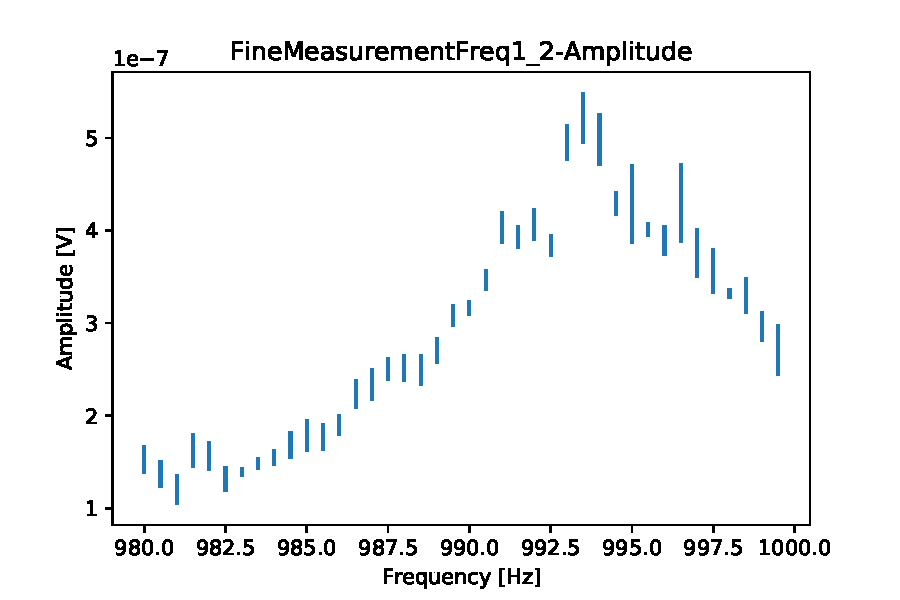
\includegraphics[width=0.45\textwidth]{figures/FineMeasurementFreq1_2amp.pdf}
	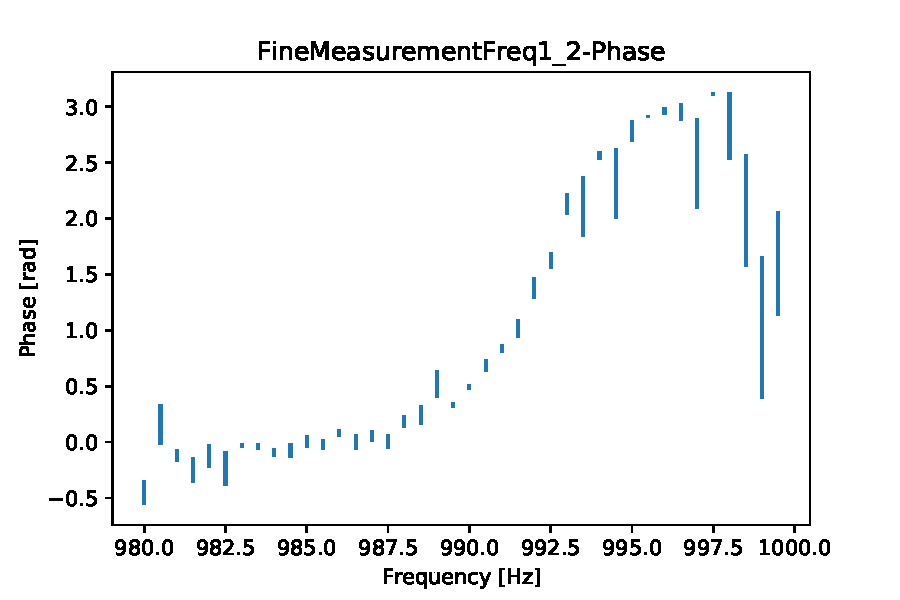
\includegraphics[width=0.45\textwidth]{figures/FineMeasurementFreq1_2phase.pdf}
	\caption{\emph{Left:} Measurement of the amplitude around the first order resonance frequency, \emph{Right:} Measurement of the phase around the first order resonance frequency}
	\label{fig4}
\end{figure}
\begin{figure}[h]
	\centering
	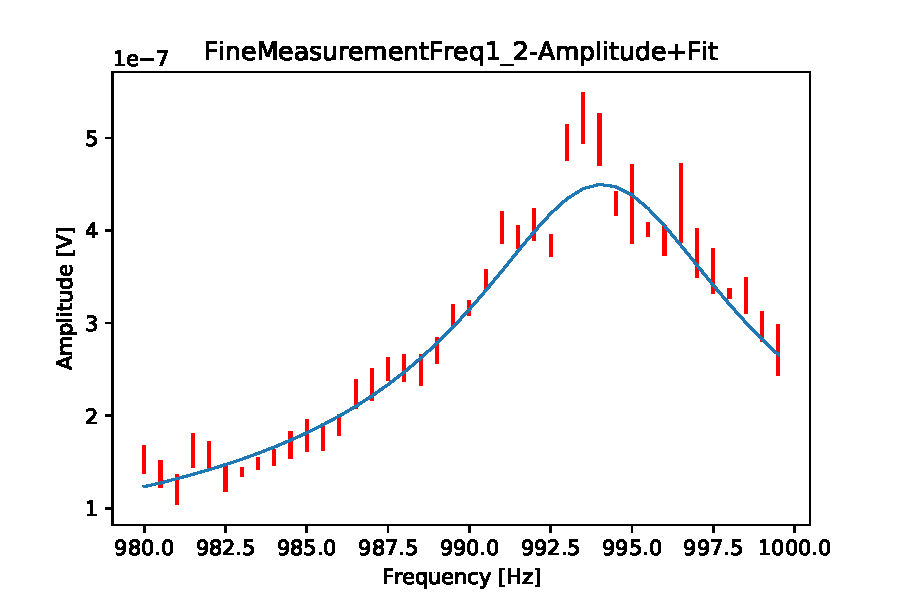
\includegraphics[width=0.45\textwidth]{figures/FineMeasurementFreq1_2fit.pdf}
	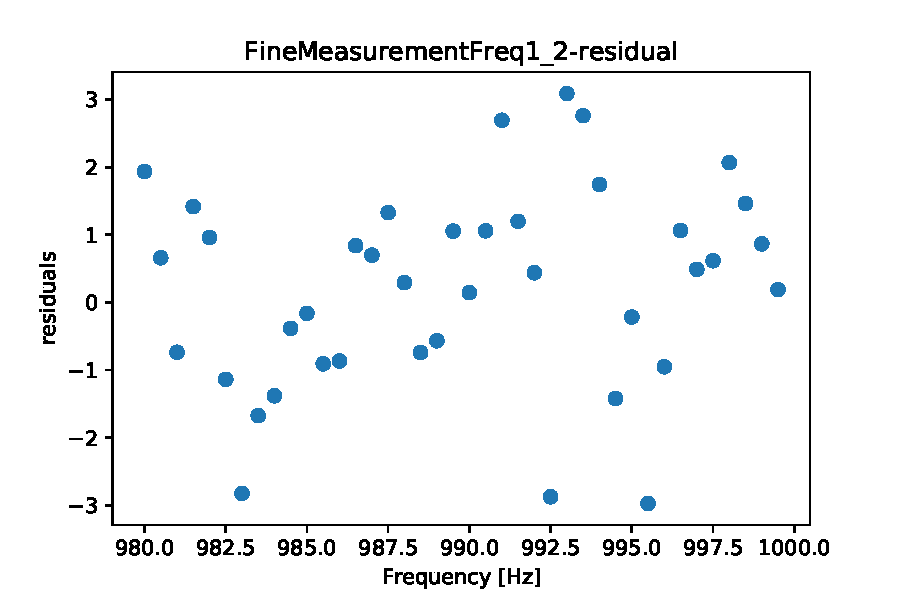
\includegraphics[width=0.45\textwidth]{figures/FineMeasurementFreq1_2residuals.pdf}
	\caption{\emph{Left:} Lorenz-fit to the data, \emph{Right:} Residuals}
	\label{fig5}
\end{figure}
\begin{figure}[h]
	\centering
	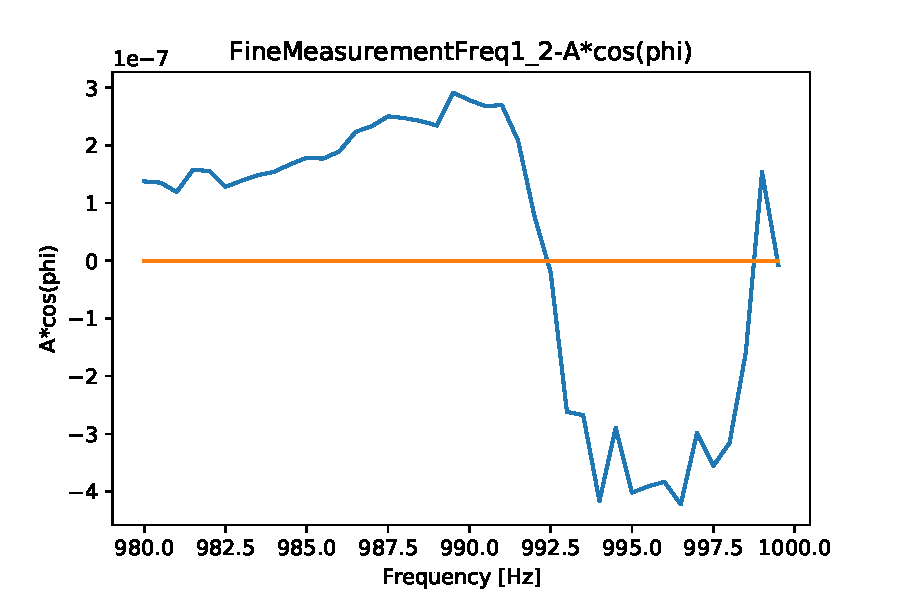
\includegraphics[width=0.45\textwidth]{figures/FineMeasurementFreq1_2acos.pdf}
	\caption{$A \cos \phi$}
	\label{fig6}
\end{figure}

\subsection{Second order resonance curve}
Unfortunately the second order resonance was not possible to detect, probably due to noise. The measurement in the region where we expected the resonance can be seen in Fig.\,\ref{fig7}

\begin{figure}[h]
	\centering
	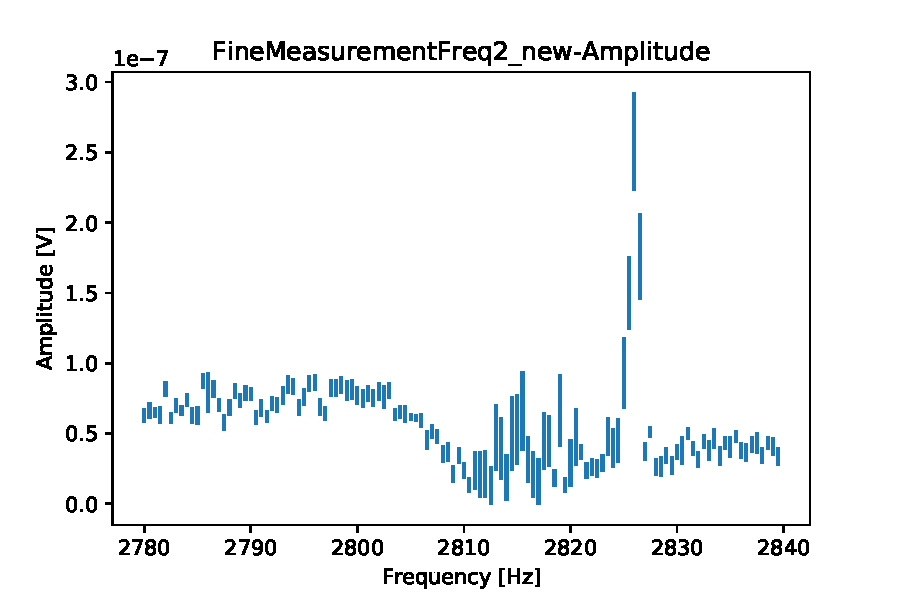
\includegraphics[width=0.45\textwidth]{figures/FineMeasurementFreq2_newamp.pdf}
	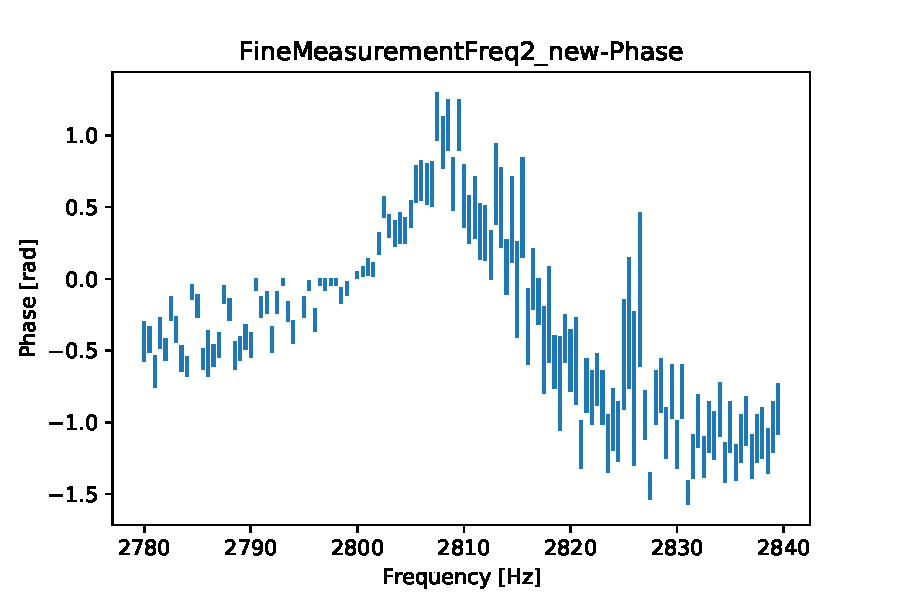
\includegraphics[width=0.45\textwidth]{figures/FineMeasurementFreq2_newphase.pdf}
	\caption{\emph{Left:} Measurement of the amplitude around the second order resonance frequency, \emph{Right:} Measurement of the phase around the second order resonance frequency}
	\label{fig7}
\end{figure}

\begin{figure}[h]
	\centering
	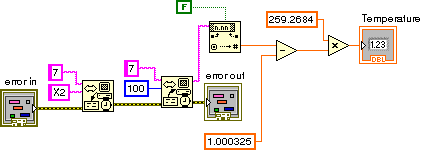
\includegraphics[width=0.45\textwidth]{figures/GetTemperatured.png}
	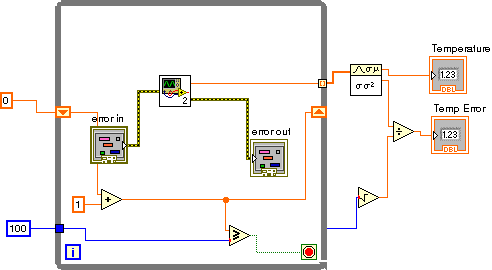
\includegraphics[width=0.45\textwidth]{figures/MeasureTemperatured.png}
	\caption{\emph{Left:} Read voltage from the Pt-1000 and convert it to a temperature, \emph{Right:} Measure the temperature 100 times (using the left module); return the mean and the error of the mean}
	\label{fig8}
\end{figure}

\begin{figure}[h]
	\centering
	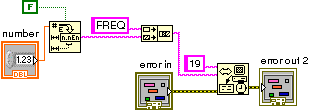
\includegraphics[width=0.45\textwidth]{figures/SetOneFreqencyd.png}
	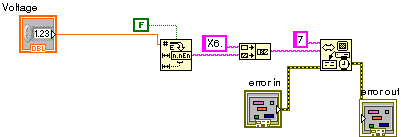
\includegraphics[width=0.45\textwidth]{figures/SetVoltaged.png}
	\caption{\emph{Left:} Set the frequency of the frequency generator, \emph{Right:} Set the voltage of the Peltier element}
	\label{fig9}
\end{figure}

\begin{figure}[h]
	\centering
	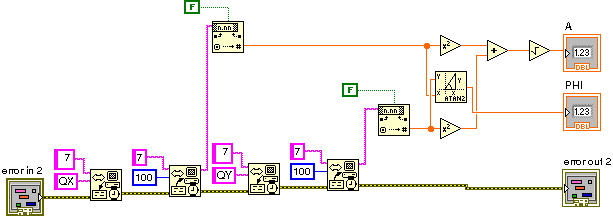
\includegraphics[width=0.45\textwidth]{figures/ReadLockInd.png}
	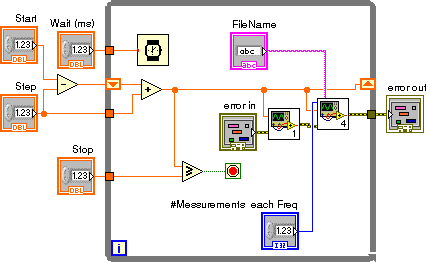
\includegraphics[width=0.45\textwidth]{figures/SetFreqRund.png}
	\caption{\emph{Left:} Read from the Lock-in amplifier. The outputs are $A\cos \phi$ and $A \sin \phi$, \emph{Right:} Measure the amplitude $A$ and the phase $\phi$ for a given frequency range.}
	\label{fig10}
\end{figure}

\begin{figure}[h]
	\centering
	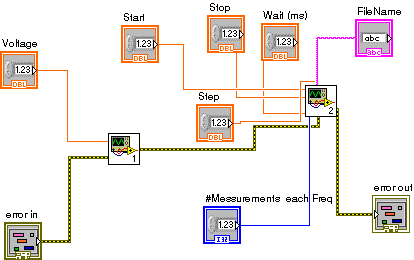
\includegraphics[width=0.45\textwidth]{figures/SetTemp__measureFreqCurved.png}
	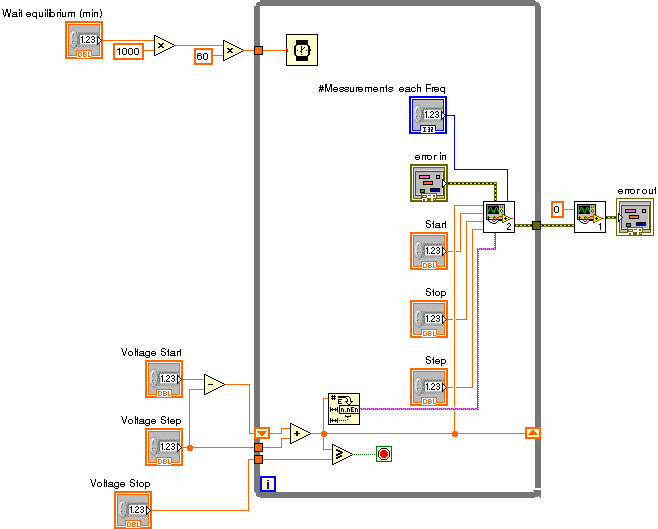
\includegraphics[width=0.45\textwidth]{figures/Maind.png}
	\caption{\emph{Left:} This module sets the voltage of the Peltier element and runs through a given frequency range to determine the resonance curve, \emph{Right:} The main module. Iterates through different voltages, waits for the equilibrium (20 min) and uses the left module to save the resonance curves for every temperature.}
	\label{fig11}
\end{figure}

\section{Temperature dependency of the resonance frequency}
In Fig.\,\ref{fig12} one can see the resonance curve of the ground resonance for different temperatures. It is clearly visible, that the temperature has an impact on the position of the peak. All those resonance curves were fitted with a lorentz curve to get the corresponding resonance frequencies and all the other relvant data as described above. The resonance frequency was then plotted against the temperature and fitted using the frequency as well as the temperature error. The program given on the course website was used to do this and we got a temperature dependency of
\begin{equation}
	\omega_0 = 2\cdot((-0.037004\pm0.00012)T+(160.790\pm0.005)).
\end{equation}  
As expected the resonance frequency dropped with higher temperatures.

\begin{figure}[h]
	\centering
	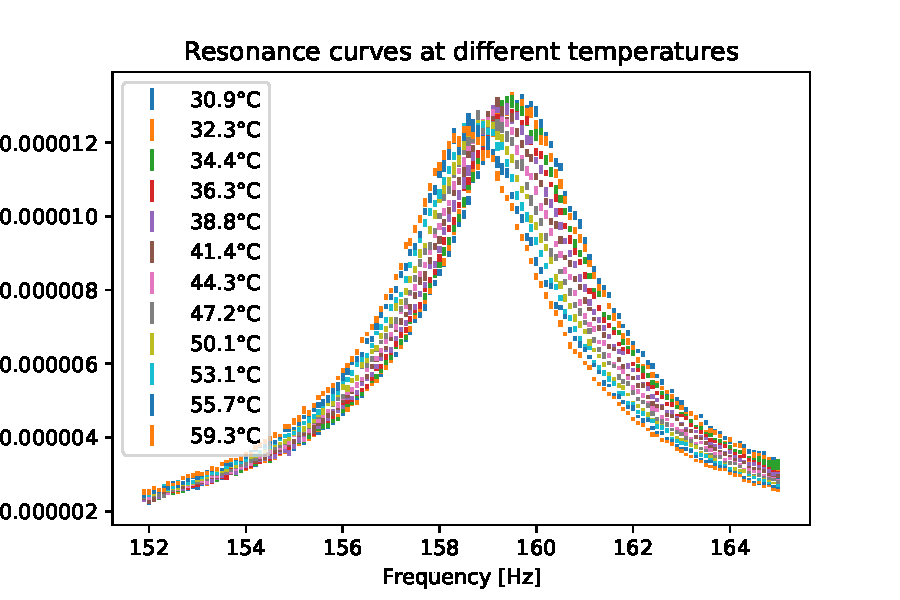
\includegraphics[width=0.45\textwidth]{figures/ResonanceTemp.pdf}
	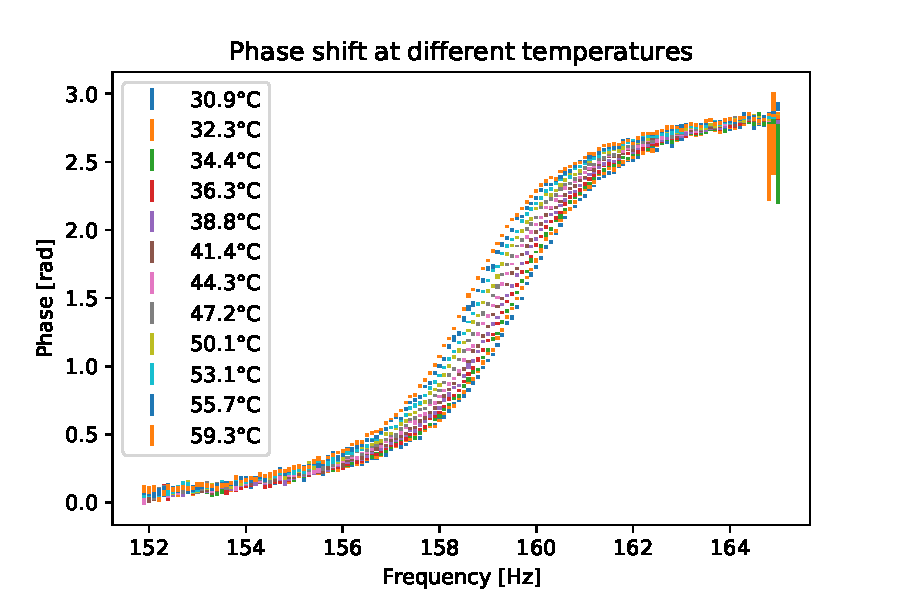
\includegraphics[width=0.45\textwidth]{figures/PhaseTemp.pdf}
	\caption{\emph{Left:} The resonance curve of different temperatures , \emph{Right:} The phase shift at different temperatures.}
	\label{fig12}
\end{figure}

\begin{figure}[h]
	\centering
	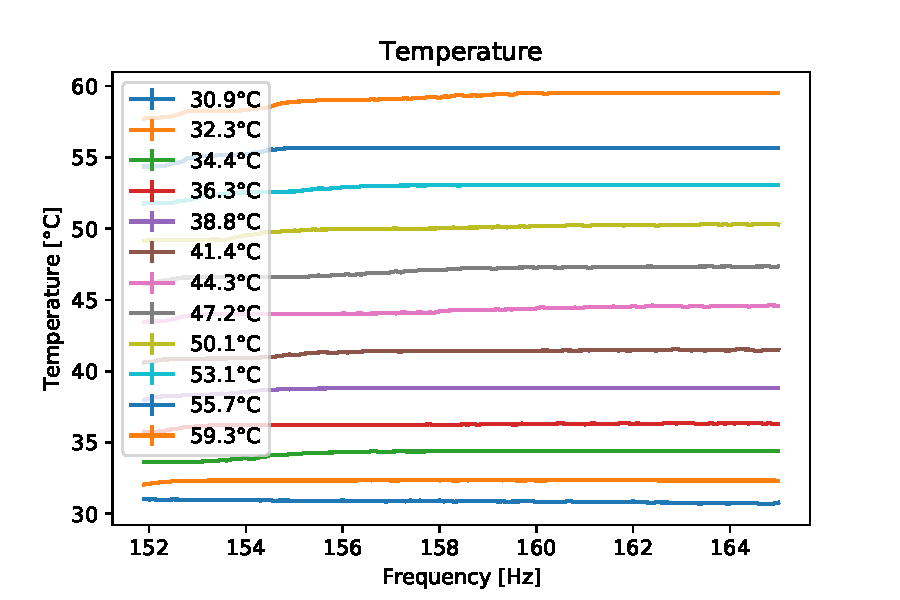
\includegraphics[width=0.45\textwidth]{figures/TempTemp.pdf}
	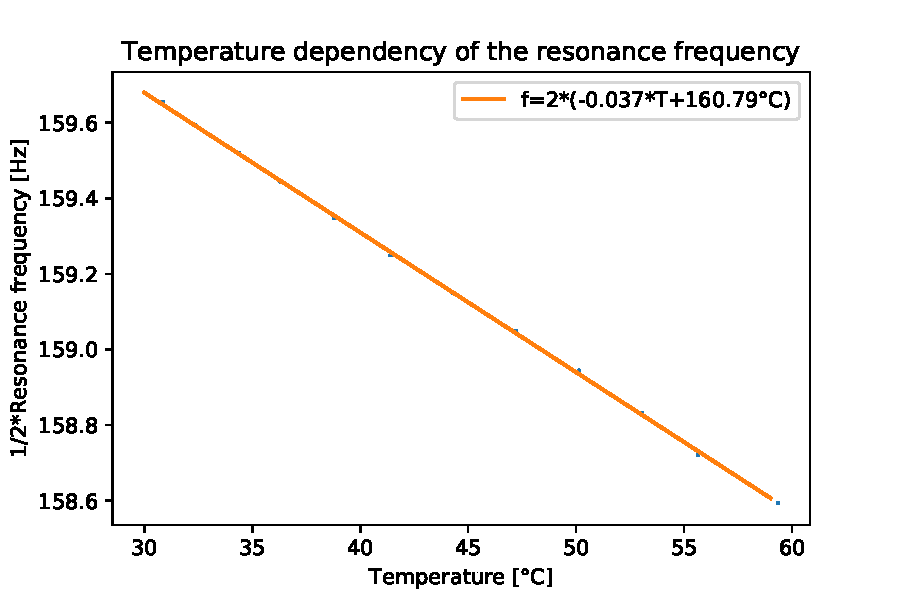
\includegraphics[width=0.45\textwidth]{figures/TempFreq.pdf}
	\caption{\emph{Left:} The measured temperatures , \emph{Right:} Temperature dependency of the resonance frequency }
	\label{fig13}
\end{figure}







